\documentclass[10pt]{article}
\usepackage[utf8]{inputenc}
\usepackage[T1]{fontenc}
\usepackage{amsmath}
\usepackage{amsfonts}
\usepackage{amssymb}
\usepackage[version=4]{mhchem}
\usepackage{stmaryrd}
\usepackage{graphicx}
\usepackage[export]{adjustbox}
\graphicspath{ {./images/} }
\usepackage{caption}

\title{PHOTOLUMINESCENCE OF METALS }

\author{A. Mooradian\\
Lincoln Laboratory,* Massachusetts Institute of Technology, Lexington, Massachusetts}
\date{}


%New command to display footnote whose markers will always be hidden
\let\svthefootnote\thefootnote
\newcommand\blfootnotetext[1]{%
  \let\thefootnote\relax\footnote{#1}%
  \addtocounter{footnote}{-1}%
  \let\thefootnote\svthefootnote%
}

%Overriding the \footnotetext command to hide the marker if its value is `0`
\let\svfootnotetext\footnotetext
\renewcommand\footnotetext[2][?]{%
  \if\relax#1\relax%
    \ifnum\value{footnote}=0\blfootnotetext{#2}\else\svfootnotetext{#2}\fi%
  \else%
    \if?#1\ifnum\value{footnote}=0\blfootnotetext{#2}\else\svfootnotetext{#2}\fi%
    \else\svfootnotetext[#1]{#2}\fi%
  \fi
}

\def\AA{\mathring{\mathrm{A}}}

\begin{document}
\maketitle
\captionsetup{singlelinecheck=false}
broad, at low temperatures is attributed by us to the coexistence of regions of pure Ta and of tantalum-impurity atom precipitates. Although ordering effects of interstitial atoms in tantaluminterstitial atom alloys previously have been observed, ${ }^{7-9}$ in the present case the concentrations of interstitial atoms were significantly lower (estimated to be: $\mathrm{N},<40 ; \mathrm{O},<100 ; \mathrm{H}, \leqslant 20 ; \mathrm{C},<40$, in ppm).

The large, sharp maxima seen at 142, 185, 205 , and 230 K in Fig. 2 may be qualitatively understood as due to ordering transitions of several impurity species. The differing lattice parameters of Ta and of Ta-interstitial-atom precipitate produce large strains at the boundaries of precipitate "clusters." Near a transition temperature clusters are rapidly fluctuating in size, and large numbers of Ta nuclei "see" the cluster boundaries. It is known that the linewidth of the NAR line in Ta is markedly dependent on strains present in the lattice. ${ }^{10,11}$ This strain sensitivity of the linewidth, combined with the density fluctuations near a transition temperature, produces a maximum in the NAR linewidth.

We acknowledge helpful comments by J. G.

Miller and J. Mishory.

\footnotetext{*Research sponsored in part by the National Science Foundation under Grant No. GP 7931, and Air Force Office of Scientific Research, U. S. Air Force, under Grant No. 65-0841.\\
${ }^{1}$ H. Suzuki and S. Miyahara, J. Phys. Soc. Japan 21, 2735 (1966), and references therein.\\
${ }^{2}$ D. G. Westlake, Phil. Mag. 16, 905 (1967), and references therein.\\
${ }^{3}$ D. G. Westlake, Trans. Met. Soc. AIME 239, 1341 (1967).\\
${ }^{4}$ D. I. Bolef, J. Appl. Phys. 32, 100 (1961). The V(I) of the present paper is the same as V(I) of this reference.\\
${ }^{5}$ R. W. Thompson and O. N. Carlson, J. Less-Common Metals 9, 354 (1965).\\
${ }^{6}$ A. J. Malland, J. Phys. Chem. 68, 2197 (1964).\\
${ }^{7}$ B. Pederson, T. Krogdahl, and O. Stakkeland, J. Chem. Phys. 42, 72 (1965).\\
${ }^{8}$ R. E. Villagrana and G. Thomas, Phys. Status Solidi 9, 499 (1965).\\
${ }^{9}$ K. K. Kelly, J. Chem. Phys. 8, 316 (1940).\\
${ }^{10}$ E. H. Gregory, dissertation, University of California at Los Angeles, 1965 (unpublished).\\
${ }^{11}$ E. H. Gregory and H. E. Bömmel, Phys. Rev. Letters 15, 404 (1965).
}(Received 31 October 1968)

\begin{abstract}
Radiative recombination in gold, copper, and gold-copper alloys has been observed arising from transitions between electrons in conduction-band states below the Fermi level and holes in the $d$ bands generated by optical excitation.
\end{abstract}

The first observation of optically excited radiative recombination of electrons and holes in metals is reported here. This emission involves states near the Fermi energy, in contrast to the soft-x-ray emission in which the excited holes are in the deep-lying bands. The noble metals gold and copper were studied as well as goldcopper alloys, but similar results should be observed in other metals.

The luminescence was excited both by an argonion laser which produced in excess of 2 W cw in either the 4880 - or the $5145-\AA$ line and by a high pressure Hg arc lamp from which the 3000 - to $4000-\AA$ emission bands were used. Samples were in the form of ingots, single-crystal slices, or evaporated films. The spectra did not seem to be dependent on the type of sample used. Measurements were made at temperatures from 5 to\\
$300^{\circ} \mathrm{K}$. Standard Raman spectroscopy techniques were used to detect the emitted light and are described elsewhere. ${ }^{1}$

Figure 1 shows the luminescence spectra of gold at 300 and $10^{\circ} \mathrm{K}$ and copper at $300^{\circ} \mathrm{K}$ with the excitation source being the $4880-\AA$ argon laser line. The emission spectra were totally unpolarized and did not vary with polarization of the incident laser beam which is consistent with luminescence from cubic cyrstals. The spectrum on the long-wavelength side is cut off by the strong absorption near the plasma edge while the shortwavelength side is limited by the energy available from the pumping source. The emission tail on the high-energy side of the laser occurs from thermal smearing of the electron and hole distributions and in the case of gold is seen to disappear at low temperature. In order to make

\begin{figure}[h]
\begin{center}
  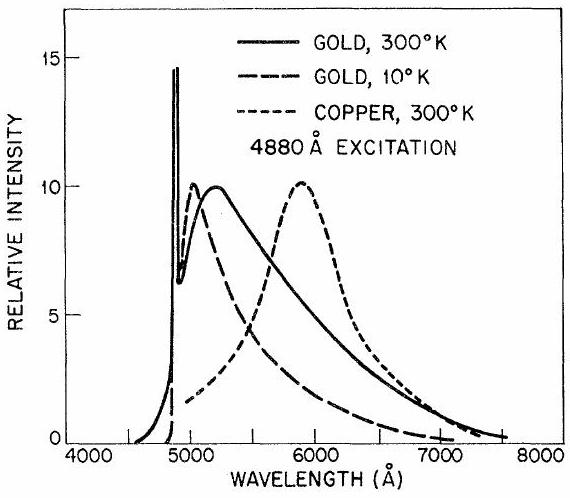
\includegraphics[alt={},max width=\textwidth]{61a709aa-f744-4cc8-aa20-36a57c58807d-2_498_570_300_292}
\captionsetup{labelformat=empty}
\caption{FIG. 1. Photoluminescence spectra of gold and copper. Exciting light was incident on the sample surface at an angle of about 10 deg from the surface while the emitted light was collected normal to the surface. The spectra are uncorrected for system response.}
\end{center}
\end{figure}

certain that the observed emission was not due to some other source such as Raman scattering from electrons, ${ }^{1,}{ }^{2}$ different excitation wavelengths of the argon laser ranging from 4579 to 5145 Å were used, as well as the 3000 - to $4000-\AA$ emission lines from a Hg arc lamp. In all cases the luminescence peaked at the same energy and the high-energy tail increased slightly with higher photon-energy pumping. There was no significant change in the emission spectrum when the angle of observation varied from forward to backward with the laser near grazing incidence. The present results are not to be confused with the optically excited plasma radiation ${ }^{3}$ reported in silver and potassium which shows no difference in frequency between the incident and emitted radiation. This plasma radiation was interpreted in terms of light scattering which involved surface roughness and which showed zero intensity for emission normal to the surface. The present results are quite unambiguous as the laser excitation provides not only a discrete exciting energy but a well-defined propagation direction and polarization. No correction was taken into account for reabsorption in the present work. Emission was also observed in copper-gold alloys which peaked at wavelengths between that for pure copper and gold. The dependence of the peak emission wavelength on alloy composition was consistent with the absorption thresholds which have been reported recently for $\mathrm{Cu}-\mathrm{Au}$ alloys. ${ }^{4}$

The details of the excitation and recombination mechanisms are shown in Fig. 2 where the band structure for a typical noble metal is represent-

\begin{figure}[h]
\begin{center}
  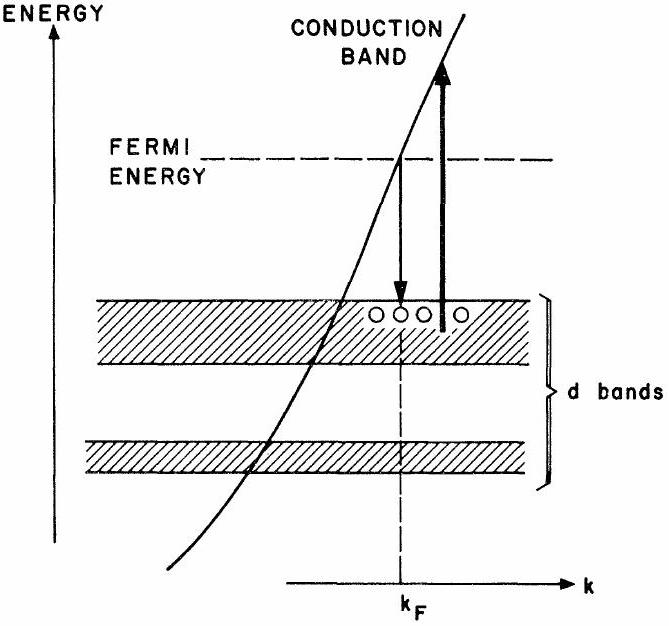
\includegraphics[alt={},max width=\textwidth]{61a709aa-f744-4cc8-aa20-36a57c58807d-2_626_669_296_1117}
\captionsetup{labelformat=empty}
\caption{FIG. 2. Schematic band structure of a noble metal showing the excitation and recombination transitions.}
\end{center}
\end{figure}

ed by a simple model which includes an $s-p$ conduction band and two sets of $d$ bands. The $d$ bands, indicated by the cross-hatched regions, in fact are made up of a number of closely lying bands in $k$ space. The interaction between the conduction band and the $d$ bands at their crossover is also neglected for simplicity. Excitation occurs from states in the upper $d$ bands to levels at and above the Fermi energy. Because of the small photon momenta the interband transitions are assumed to be direct. Indirect recombination cannot be ruled out but would have to involve the participation of a phonon or an impurity to provide the necessary momentum. If the photoexcited holes in the $d$ band thermalize before recombining, they would collect at the zone boundary since the $d$ bands slope upward slightly with increasing $k$. The radiative transitions would then have to be indirect. The onset of emission in this case would be significantly shifted to lower energy from the laser exciting line. No such shift is observed. It seems more likely that the emission arises from direct recombination of conduction-band electrons below the Fermi energy with holes in the $d$ band that have been scattered to momentum states less than the Fermi momentum, $k_{\mathrm{F}}$. Band calculations made on the noble metals such as copper ${ }^{5}$ and gold indicate that the $d$ bands can be relatively flat at some regions in $k$ space less than $k_{\mathbf{F}}$. This might allow photoexcited holes to be scattered into a sufficient range of states in $k$ space to account for the observed broad linewidths. Gold showed an appreciable sharpening and shift of its spectrum at low temperature which is attributed in part to a\\
change of the plasma absorption edge as well as narrowing of the distribution of electrons and holes. The copper spectrum also narrowed slightly and shifted from 5930 to about $5800 \AA$ in going from 300 to $10^{\circ} \mathrm{K}$.

The intensity of recombination radiation for direct transitions between electrons and holes is given by ${ }^{6}$


\begin{equation*}
I(h \nu) \propto \nu^{2} \int_{S}|M(\overrightarrow{\mathrm{k}})|^{2} f e^{(\overrightarrow{\mathrm{k}}) f} h^{(\overrightarrow{\mathrm{k}})} \frac{d S}{\left|\nabla_{k}\left(\epsilon_{e}^{-\epsilon} h\right)\right|} \tag{1}
\end{equation*}


Here $I(h \nu)$ is the intensity per unit range of photon energy, $M$ is the interband matrix element, $f_{e}(\overrightarrow{\mathrm{k}})$ and $f_{h}(\overrightarrow{\mathrm{k}})$ are, respectively, the electron and hole distribution functions which may not be uniform in space, and $S$ is the surface corresponding to the energy $\epsilon_{e}(\overrightarrow{\mathrm{k}})-\epsilon_{h}(\overrightarrow{\mathrm{k}})=h \nu$ in wavevector $(\overrightarrow{\mathrm{k}})$ space. Because the line shape involves the energy-momentum relation of the various bands, the spectra might help to elucidate the band structure of these metals. The role of excitons in the recombination has been neglected since the high electron densities should effectively screen out any exciton bound state. However, there has been some speculation ${ }^{7}$ about the existence of excitons in metals and perhaps the luminescence studies would help to demonstrate this effect.

In both metals the peak emission was consistent with the optically observed energy between the upper $d$ band and the Fermi energy ${ }^{8}$ : 2.0 eV for copper and 2.2 eV for gold. Similar transitions between the conduction band and the lower $d$ band should also be observed for sufficiently high pump energies. The transitions should occur around 4 eV . Further experiments are in progress to observe this transition. The maximum integrated efficiency of recombination ne-\\
glecting corrections for reabsorption was estimated to be on the order of 1 part in $10^{10}$.

The observation of interband radiative recombination in metals may very well provide another technique to help investigate some properties of the band structure of metals as well as to determine the nature of scattering mechanisms of excited electrons and holes. Photoluminescence might also be observed for transitions between higher lying bands in semiconductors and semimetals and could be accessible to study by laser excitation techniques.

The author would like to thank Dr. G. F. Dresselhaus for many informative discussions and Mr. D. J. Wells for assistance with the measurements.\\
*Operated with support from the U. S. Air Force.\\
${ }^{1}$ A. Mooradian, Phys. Rev. Letters 20, 1102 (1968).\\
${ }^{2}$ A. Mooradian, in Proceedings of the International Conference on Light Scattering from Solids, New York, 1968 (to be published).\\
${ }^{3}$ For a review article on this effect which contains pertinent references, see W. Steinmann, Phys. Status Solidi 28, 437 (1968).\\
${ }^{4}$ P. O. Nilsson, A. Persson, and S. Hagström, Solid State Commun. 6, 297 (1968).\\
${ }^{5}$ G. A. Burdick, Phys. Rev. 129, 138 (1963); B. Segall, Phys. Rev. 125, 109 (1962); E. C. Snow and J. T. Waber, Phys. Rev. 157, 570 (1967); H. L. Davis, J. S. Faulkner, and H. W. Joy, Phys. Rev. 167, 601 (1968); E. C. Snow, Phys. Rev. 171, 785 (1968).\\
${ }^{6}$ A. Mooradian and H. Y. Fan, Phys. Rev. 148, 873 (1966).\\
${ }^{7}$ M. H. Cohen, in Optical Properties and Electronic Structure of Metals and Alloys, edited by F. Abelès (North-Holland Publishing Company, Amsterdam, The Netherlands, 1966), p. 66.\\
${ }^{8}$ D. Beaglehole, Proc. Phys. Soc. (London) 85, 1007 (1965), and 87, 461 (1966).


\end{document}